\documentclass{beamer}

% For more themes, color themes and font themes, see:
% http://deic.uab.es/~iblanes/beamer_gallery/index_by_theme.html
%
\mode<presentation>
{
  \usetheme{Madrid}       % or try default, Darmstadt, Warsaw, ...
  \usecolortheme{crane} % or try albatross, beaver, crane, ...
  \usefonttheme{serif}    % or try default, structurebold, ...
  \setbeamertemplate{navigation symbols}{}
  \setbeamertemplate{caption}[numbered]
} 

\usepackage{tikz}
\usetikzlibrary{decorations.markings,angles}
\usepackage{tikz-3dplot} 
\usepackage{floatrow}
\usepackage{amsmath}


\begin{document}



\begin{frame}{Magnetic field measurements}

\begin{itemize}
\item azimuth of the magnetic field from linear polarization(ambiguity in orientation): 

$\phi$ = 0.5 arctan(U/Q)

\item strength of L.O.S  magnetic field from zeeman shift
\end{itemize}
First vector
magnetic field inferences along an individual, resolved coronal
loop structure extending up to heights of 70 Mm (0.1 RSun ) and
the first polarimetric measurements of coronal loops located {\bf on
disk}

Off-limb studies in
optically thin spectral lines must take into account LOS
integration effects

\end{frame}

\begin{frame}{Other off limb magnetic field measurements}
 
\begin{figure}[H]
 \centering
 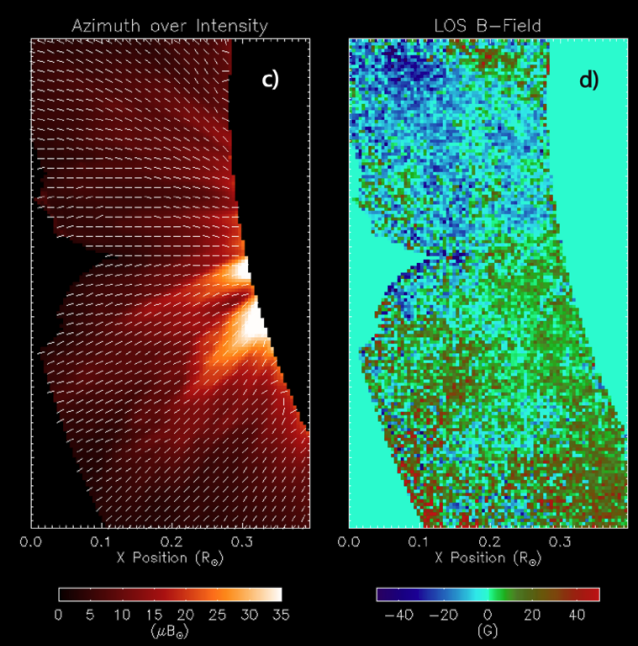
\includegraphics[scale=0.27]{t1c.png}
\caption{Tomczyk et al. 2008 measurements: left intensity with superimposed vectors showing the plane of sky direction
of the magnetic field, right: the LOS component of the magnetic field}
\end{figure}
\end{frame}



\begin{frame}{Other off limb magnetic field measurements}

\begin{figure}[H]
 \centering
 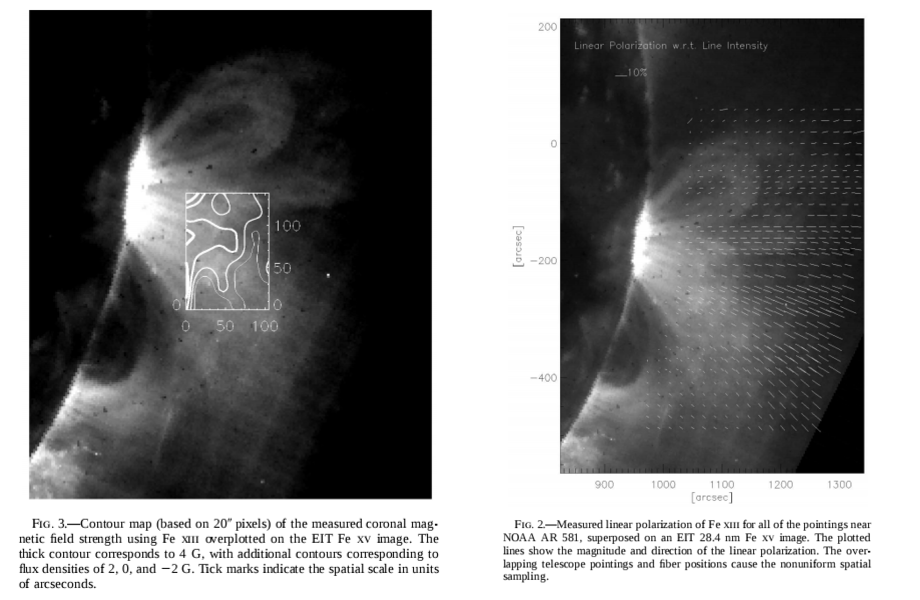
\includegraphics[scale=0.32]{lin.png}
\caption{Lin et al. 2004 measurements (100 arcsec $\approx$ 72.5 Mm)}
\end{figure}


\end{frame}

\begin{frame}{Magnetic field measurements from seismology}
\begin{figure}[H]
 \begin{minipage}[c]{0.5\textwidth}
    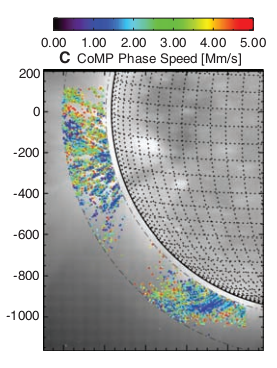
\includegraphics[scale=0.5]{ts4.png}
  \end{minipage}\hfill
  \begin{minipage}[c]{0.5\textwidth}
    \caption{
Tomczyk et al. 2007 performed coronal seismology techniques  to off-limb observations of
the Fe XIII line (at projected heights above 35 Mm) and
inferred average coronal magnetic field strengths between 8
and 26 G using the Alfv\'en wave phase relation:
\newline
1) using relationship $v_A=\frac{B}{\sqrt{\mu_0 \rho_c}}$
\newline 2)measuring phase speed between 1.2 and 5 Mm/s
(Alfv\'en waves are incompressible, so they
are not visible as intensity fluctuations,
velocity fluctuations
inferred from Doppler shifts of emission)
\newline 3)using typical electron density of $10^8 /cm^3$
    } 
  \end{minipage}
\end{figure}


\end{frame}


\begin{frame}{Magnetic field measurements from seismology}
Comparison of wave propagation angle with azimuth angle of magnetic field determined from linear polarization measurement
(angles relative to solar north-south)
\begin{figure}[H]
  \begin{minipage}[c]{0.33\textwidth}
    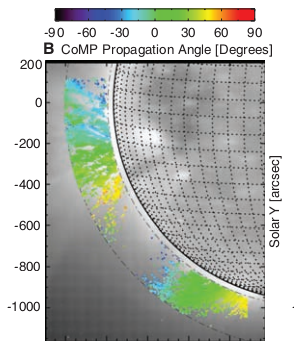
\includegraphics[scale=0.4]{ts2.png}
  \end{minipage} \hfill
 \begin{minipage}[c]{0.33\textwidth}
    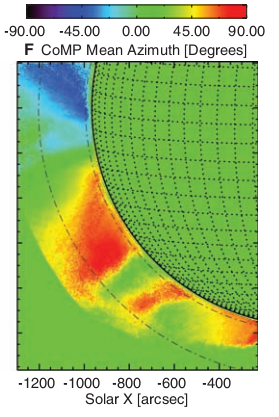
\includegraphics[scale=0.4]{ts1.png}
  \end{minipage}\hfill
 \begin{minipage}[c]{0.33\textwidth}
    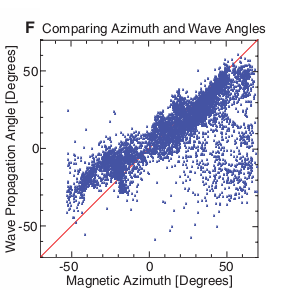
\includegraphics[scale=0.4]{ts3.png}
  \end{minipage}
\end{figure}

\end{frame}


\begin{frame}{Magnetic field measurements from gyrofrequency}

\begin{figure}[H]
 \begin{minipage}[c]{0.3\textwidth}
    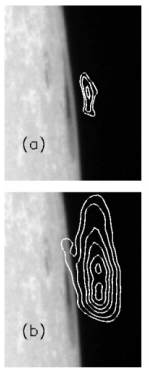
\includegraphics[scale=0.6]{bw1.png}
  \end{minipage}\hfill
  \begin{minipage}[c]{0.7\textwidth}
    \caption{
			Brosius, White, 2006 determine magnetic field strength by measuring cyclotron frequency of electrons at 15Ghz and 8Ghz
			 (a) 15 GHz radio intensity contours of 1.5, 3.0, and 6.0 $\cdot 10^5$ K; 
			(b) 8 GHz radio intensity contours of 0.125, 0.25, 0.5, 0.75, 1.0 and 1.25 $\cdot 10^6;$ K
			\newline1) calculate free-free radio brightness temperature at the location of 15Ghz peak: $3.4 \cdot 10^4  K \ll 6.9 \cdot 10^5K$ observed
			\newline 2)2 observed peaks for brightness temperature 8Ghz  $1.3 \cdot 10^6$, $1.4\cdot 10^6$ K  $\gg 6\cdot 10^4$K calculated
			\newline 3) conclude that emission comes mainly from cyclotron
			\newline	4)use formula  $f = \frac{e B}{m_e} \frac{m}{2\pi}$ (m is harmonic number?), conclude that m should be 3 and 
			obtain B = 1750G for the 15Ghz peak location(8Mm) and 960G for  the 8Ghz peak location (12Mm above umbral center)
    } 
  \end{minipage}
\end{figure}

\end{frame}


\begin{frame}{Magnetic field measurements }

\begin{itemize}
\item cool, neutral material measured in this observation
\item upper temperature 15000 - 35000K determined from Doppler widths (in the same HeI line) in accordance with measurements by Ahn
and Antolin which found that coronal rain is a multithermal phenomenon with a spatially
thin transition between chromospheric and TR temperatures.
Meanwhile, their observations suggest a relatively wider, yet
still narrow, transition (0.5arcsec) from TR to coronal
temperatures
\item lower level of HeI maintained by recombination(electrons captured by HeIII and HeII ions) and rapid deexcitation cascade $\implies$
the line formation is linked to the availability of ions tied to the
magnetic field (similar discussion as in the case of $H\alpha$ line by Antolin and Rouppe van de Voort in order to explain 
why we expect neutral material to trace the magnetic field)
\end{itemize}
\end{frame}

\begin{frame}{Partial ionization effects}
\begin{figure}[H]
 \centering
 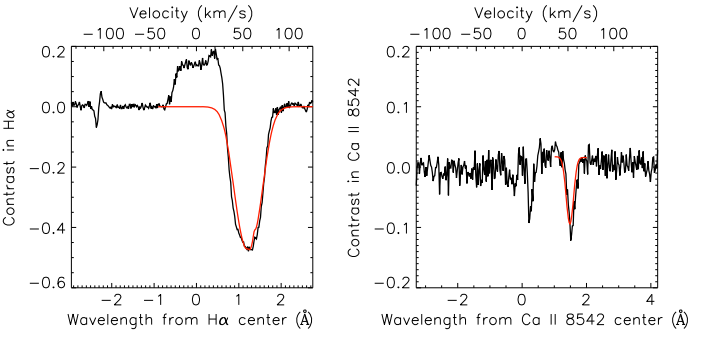
\includegraphics[scale=0.32]{ahn1.png}
\caption{Ahn 2014 measurements showed neutral
and ionized species to fall in unison}
\end{figure}

\end{frame}

\begin{frame}{Partial ionization effects}
ions and neutrals decoupled which may lead to cross field diffusion

\begin{figure}[H]
 \begin{minipage}[c]{0.6\textwidth}
    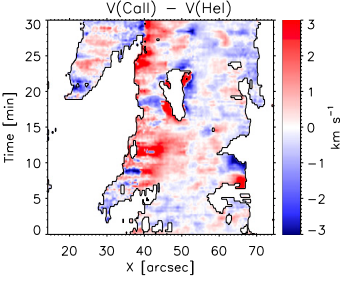
\includegraphics[scale=0.45]{kh2016.png}
  \end{minipage}\hfill
  \begin{minipage}[c]{0.4\textwidth}
    \caption{
			Khomenko et al 2016 measurements showed small differences between neutrals and ions velocities in a solar prominence
    } 
  \end{minipage}
\end{figure}

Gilbert et al. (2002) calculated the neutral helium cross-field
downflow speed to be $8 \cdot 10^3$ cm/s , while values reached
10 km /s for prominence material of very low density
($10^9 cm^-3$ ), both of which are small fractions of the velocities
observed here 

\end{frame}


\begin{frame}{Condensation effects}

\begin{figure}[H]
    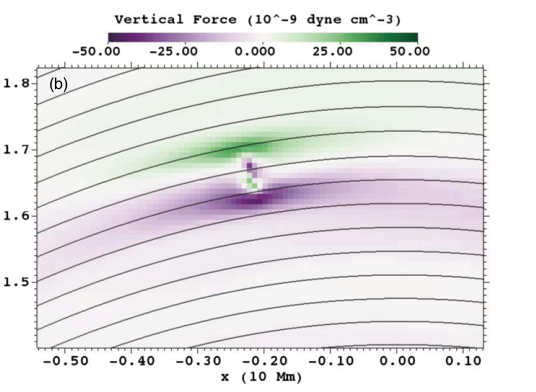
\includegraphics[scale=0.4]{fang1.png}
    \caption{
Fang et al. (2013) determined that the
pressure gradient brought on by the formation of small, but
dense, coronal condensates introduces a force on par with the
Lorentz force, and thus the presence of the cool material can
induce field variations locally and within its neighborhood
    } 
\end{figure}

\end{frame}


\begin{frame}{Future improvements}
\begin{itemize}
\item  Daniel K. Inouye Solar Telescope:

substantial increase of light-gathering capability
\item 
new diagnostics techniques such as the use of the He I polarization as a
height diagnostic Asensio Ramos et al. 2008: 

determining consistently the height-dependent atomic level polarization induced by the anisotropic radiation field
within the atmosphere model that provides the best fit to the observed
Stokes profiles. Since the anisotropy factor is very sensitive
to the source function gradient  the solution of these types of problems in stratified model
atmospheres may be facilitated by the application of efficient iterative
schemes
\end{itemize}


\end{frame}


\end{document}
